% Virtualization chapter about concept, types, examples and implementation
\label{chapter:virtualization}

Jak je z názvu kapitoly patrné, hlavním obsahem následující části práce bude virtualizace a to především odvětví, které se věnuje výpočetní technice. Virtualizace je velice komplexní téma, a proto je nutné řádně
specifikovat z jakého úhlu pohledu se na toto téma koukáme.

Po představení obecného konceptu virtualizace se proto podíváme na několik oblastí využité této technologie v informačních technologiích. Detailní popis všech oblastí virtualizace není předmětem této práce, a proto
se ve zbytku diplomové práce budeme věnovat pouze tématu virtualizace serverů. I takto specifikované téma ale obsahuje mnoho virtualizačních principů a technik, které si u jednotlivých typů virtuálních strojů představíme.
Jelikož virtualizace zažívá v dnešní době velký rozvoj, podíváme se také na jednotlivé scénáře nasazení serverů využívající virtualizaci. V poslední části této kapitoly jsou blíže představeny vybrané principy
virtualizace a základy virtualizace CPU, paměti a I/O zařízení. TODO (uvidíme jestli bude třeba popisovat vše)

\section{Obecná definice virtualizace}
\label{section:virtualization:definition}

Než se pustíme do popisu jednotlivých typů virtualizace detailněji, je vhodné definovat tento pojem v obecném slova smyslu. Slovo virtuální je dle \cite{oxford:dictionary:virtual} definováno následovně.

\begin{definition}[Virtual]
  \label{definition:virtual}
  Almost or nearly as described, but not completely or according to strict definition.
\end{definition}

Ve výpočetní technice má tento výraz podle stejného zdroje \cite{oxford:dictionary:virtual} podobnou definici.

\begin{definition}[Virtual in computing]
  \label{definition:virtual_computing}
  Not physically existing as such but made by software to appear to do so.
\end{definition}

Proces virtualizace ve výpočetní technice tedy můžeme definovat jako vytváření virtuálních prostředků, které skrývají nebo upravují podstatu fyzických prostředků před uživatelem. Tento proces zahrnuje vytváření více
virtuálních prostředků z jednoho fyzického. Jako příklad této virtualizace můžeme použít virtuální paměť, kdy se virtuální paměť více procesů mapuje do hlavní (fyzické) paměti počítače. Na druhou stranu může jít i o
vytvoření jednoho virtuálního prostředku z více fyzických prostředků. Příkladem pro tento typ virtualizace může být vytvoření jednoho logického disku z několika fyzických a to například v konfiguraci RAID. 

Virtualizace si zcela jistě objevuje i v jiných oblastech, ale nás bude zajímat, jak se tento koncept využívá k virtualizaci výpočetní techniky a konkrétně jeho využití v sítích, operačních systémech a také 
v počítačovém HW. 

\section{Virtualizace ve výpočetní technice}
\label{section:virtualization_in_it}

Virtualizace se v dnešní době stala důležitou součástí návrhu počítačových systémů a zdárně se využívá v mnoha oblastech informačních technologií. Velkého rozvoje dosáhla především v oblastech virtualizace operačních
systémů, procesorů, sítí ale také programovacích jazyků.

Pokud se podíváme na architekturu dnešních počítačových systémů z pohledu struktury a typů zařízení, které se v ní vyskytují, můžeme najít hned několik oblastí ve kterých se virtualizace využívá. 

  \subsection{Virtualizace serverů}
  \label{subsection:server_virtualization}
  
  V dnešní době je pro většinu společností téměř nutností nějakým způsobem využívat výpočetních prostředků. Důvod pro jejich použití může být potřeba ukládání a zálohy obchodních záznamů, poskytování interních nebo
  externích služeb či běh výpočetně náročné aplikace. Ať tak či onak, hlavním poskytovatelem výpočetního výkonu v dnešních počítačových systémech je výpočetní server.
  
  Klasický výpočetní server je fyzický počítač (HW), který poskytuje své výpočetní prostředky řídícímu programu. Řídícím programem se klasicky myslí operační systém. Druhy serverů můžeme rozdělit dle typu běžících
  uživatelských programů v operačním systému. Konkrétně pak hovoříme o aplikačních, souborových nebo výpočetních serverech, které se specializují na poskytování různých druhů služeb, jak je patrné z jejich názvu.
  
  Proces virtualizace serverů spočívá v přenesení operačního systému a jeho služeb do virtuálního prostředí, které napodobuje chování HW ale není závislé na nižších vrstvách. Dochází tedy ke zvýšení přenositelnosti a
  možnosti současného běhu více instancí OS na jednom fyzickém stroji. Vytváření toho virtuálního prostředí je zajištěno speciální softwarovou vrstvou zvanou virtualizační monitor, hraje roli řídícího programu a
  pracuje mezi HW a jednotlivými instancemi OS. Virtualizační monitor nebo také VMM je detailněji popsán v kapitole \ref{section:vmm}, kde jsou představeny jeho hlavní funkce a jednotlivé typy.
  
  Počítačové systémy využívající virtualizace se skládají z dalšího typu serverů tzv. virtualizačních serverů, které slouží jako zdroj fyzických prostředků pro instance OS a jejich uživatelské programy. Tyto servery
  se vyznačují především velkým množstvím operační paměti a vysokým výpočetním výkonem, který je díky VMM rozdělován mezi hostované operační systémy. Výhody nasazení virtuální infrastruktury jsou dále popsány v
  kapitole \ref{section:vm_deployment}.

  Tato práce se zaměřuje právě na techniky virtualizace, které jsou v dnešní době aktuální a využívají se k virtualizaci serverů. Práce podrobně představuje virtualizační techniku Solaris Zones of firmy Oracle,
  která slouží pro vyváření virtuálních strojů (zón), které sdílejí jedno jádro OS.

  \subsection{Využití virtualizace v sítích}
  \label{subsection:network_virtualization}

  Oblast komunikačních sítí je další neméně významnou oblastí pro využití virtualizačních technik. Bez síťové infrastruktury by mezi sebou počítače nemohli komunikovat, a tudíž by jejich využití nemělo takový potenciál.
  V dnešní době je tato infrastruktura značně rozsáhlá a to v některých případech ztěžuje její správu. S virtualizací přichází do sítí možnost dynamické konfigurace sítě a to i její topologie. To vše lze uskutečnit z 
  jednoho místa a bez nutnosti zasahovat do fyzických zařízení sítě.

  Virtualizace sítí je koncept, který se v mnoha ohledech podobná virtualizaci serverů. V případě serverů, se VMM stará o reprodukci vlastností fyzických prostředků v SW. Podobně je to tomu i v případě virtualizace sítí,
  kde existuje funkční ekvivalent VMM, který reprodukuje síťové komponenty v SW. Administrátor má tak možnost za chodu vytvářet virtuální síťové komponenty jako je switch, router, firewall nebo load balancer a to vše v
  rámci desítek sekund. Tento síťový VMM také umožňuje spravovat nové virtuální sítě, které zahrnují všechny standardní síťové služby a kvalitu služeb.\cite{article:vmware:network_virtualization}

  \subsection{Virtualizace desktopu}
  \label{subsection:desktop_virtualization}
  
  Společně s virtualizací serverů a sítí je virtualizace desktopu posledním typem virtualizace, která stojí za zmínku. Pod pojmem desktop si představme klasický stolní počítač, který má obrazovku, myš a klávesnici.

  S desktopem je klasicky spojeno grafické uživatelské prostředí, pomocí kterého uživatel ovládá počítač, instaluje aplikace nebo přizpůsobuje prostředí. Bez využití virtualizace nebo další podpůrných systémů jsou 
  všechny informace o uživatelském nastavení uloženy na desktopu a uživatel se k nim dostane pouze z toho samého stroje. Virtualizací desktopu je rozuměno oddělení uživatelského prostředí a nastavení od fyzického
  stroje. Jednou z možností je přesunutí tohoto prostředí do virtuálního stroje, který je centrálně spravován a spouštěn, když uživatel potřebuje. Tento koncept umožňuje uživateli přístup ke svému prostředí téměř
  bez ohledu na lokalitu nebo platformu. Mezi další benefity zavedení virtualizovaného desktopu patří zvýšení bezpečnosti a zjednodušení správy celého systému. Tyto výhody pramení především z centralizaci tohoto
  řešení.
  

  
\section{Virtuální stroj}
\label{section:virtual_machine}

V části \ref{section:virtualization:definition} jsme si definovali virtualizaci obecně jako virtualizaci fyzických (HW) prostředků.  Virtualizace systému nebo komponenty jako je procesor, paměť nebo I/O zařízení na určité vrstvě
architektury počítače znamená mapování jeho rozhraní na rozhraní nižší vrstvy způsobem, který může reprezentovat v jiném smyslu než fyzicky existuje.

Tento koncept virtualizace nemusí být aplikován pouze na jednotlivé subsystémy jako například disky, ale může být zobecněn na celý systém. Pro tento účel je zavedena speciální SW vrstva, která operuje mezi konkrétními
vrstvami počítačového systému, aby bylo dosaženo požadované architektury. Tato vrstva poskytuje vyšším vrstvám rozhraní a všechny prostředky nižší vrstvy tak, že vyšší vrstvy nemají o existenci této vrstvy ponětí a přitom
dochází k virtualizaci celého systému. Tímto způsobem může virtuální stroj obejít kompatibilitu některých komponent fyzického stroje nebo omezení HW prostředků.

Než budeme pokračovat s klasifikací virtuálních strojů, představíme si architekturu klasického počítačového systému.

  \subsection{Architektura počítačového systému}
  \label{subsection:computer_architecture}
  
  Jelikož implementace virtuální strojů operují na rozhraních jednotlivých vrstev architektury počítačového systému, je nutné se řádně s těmito vrstvami seznámit. Tyto vrstvy reprezentují několik úrovní abstrakce v
  počítačovém systému, které mají za úkol odstínit složité implementační detaily některých rozhraní. Čím výše se v této hierarchii nacházíme, tím abstraktnější a jednodušší funkce máme k dispozici.
  
  Každá z vrstev má dobře definované rozhraní, což umožňuje vývoj vyšších vrstev nezávisle na implementaci nižších vrstev, pokud tyto vrstvy budou dodržovat toto rozhraní. Jako příklad si můžeme vzít výrobce procesorů
  Intel a AMD vyrábějící mikroprocesory, které implementují instrukční sadu IA-32 (x86) \cite{book:iee:vm_architecture}. Zatímco nezávisle na vývoji těchto procesorů můžou vývojáři softwaru vyvíjet aplikace, které
  se kompilují do této instrukční sady. Takto zkompilovaný program pak může být bez problému spuštěn na každém počítači s procesorem architektury IA-32.
  
  Na druhou stranu komponenty navržené pro jeden typ rozhraní nebudou fungovat s rozhraním jiného typu. Jednoduše řečeno program sestavený pomocí instrukcí x86 se nebude dát spustit na počítači s procesorem architektury
  SPARC. Nicméně díky některým technikám virtualizace se tohoto dá dosáhnout. 
  
  Obrázek \ref{figure:computer_architecture} ukazuje hierarchii počítačového systému a některé jeho SW i HW vrstvy. Dále jsou na obrázku vyznačeny následující rozhraní.
  
  \begin{itemize}
   \item Instruction set architecture - ISA
   \item Application binary interface - ABI
   \item Application programming interface - API
  \end{itemize}

  Tyto tři rozhraní jasně definují rozmezí mezi HW a SW a určují architekturu počítačového systému. Uživatelské programy jsou zcela odkázány na funkcionalitu, která je jim poskytnuta kombinací těchto rozhraní.

    \begin{figure}
      \centering
      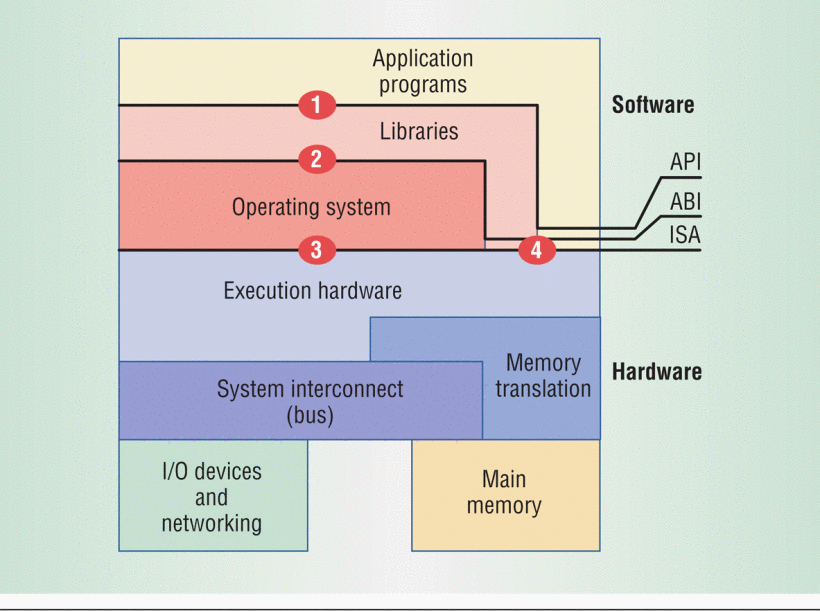
\includegraphics[scale=0.3]{assets/figures/ca.png}
      \caption[Architektura počítačového systému]{Architektura počítačového systému \cite{book:iee:vm_architecture}}
      \label{figure:computer_architecture}
    \end{figure}


    \subsubsection*{Instruction set architecture}
    \label{subsubsection:isa}
    
    Instrukční sada neboli ISA definuje rozhraní mezi HW a SW. Rozdělit jí můžeme na dvě části a to na systémovou a uživatelskou instrukční sadu. Rozhraní s číslem 4 na obrázku \ref{figure:computer_architecture}
    reprezentuje uživatelskou instrukční sadu, která obsahuje instrukce dostupné pro všechny uživatelské programy i knihovny. Rozhraní s číslem 3 na stejném obrázku pak reprezentuje systémovou instrukční sadu a zahrnuje
    instrukce dostupné pouze operačnímu systému. Tyto instrukce je možné vykonávat pouze v privilegovaném režimu procesoru a jsou zodpovědné za správu HW prostředků.

    \subsubsection*{Application binary interface}
    \label{subsubsection:abi}
    
    Fyzické prostředky a zařízení dostupné v fyzickém systému spravuje operační systém, který k nim poskytuje přístup ostatním programům skrze svoje rozhraní. Toto rozhraní (číslo 2) se nazývá systémové a společně s uživatelskou
    částí (číslo 4) tvoří tzv. \textit{application binary interface} neboli ABI. Toto rozhraní tedy neposkytuje aplikačním programům přímý přístup k HW prostředkům, ale zprostředkovává je skrze systémová volání.
    Operační systém tak 

    \subsubsection*{Application programming interface}
    \label{subsubsection:api}
    
    Důležitou vrstvou softwarového vybavení počítače jsou uživatelské knihovny. Tyto knihovny skrývají implementační detaily systémových volání a poskytují rozhraní (číslo 1) pro vyšší programovací jazyky
    jako je C nebo C++. Společně s uživatelskou částí instrukční sady (číslo 4) tvoří rozhraní nazývané \textit{application programming interface} neboli API. Uživatelské programy pak mohou využívat tohoto rozhraní,
    což přináší výhody v přenositelnosti na systémy, které nabízejí stejné API .

\section{Klasifikace virtuálních strojů}
\label{section:clasification}

Abychom mohli rozlišit jednotlivé typy virtuálních strojů, musíme se podívat v jaké části počítačové architektury operují a tedy jakou vrstvu virtualizují. V části \ref{subsection:computer_architecture} jsme definovali
tři dobře definované rozhraní počítačového systému a je logické, že virtualizační software bude virtualizovat nějakou z nich. Dle rozdělení v \cite{book:iee:vm_architecture} můžeme virtuální stroje obecně rozdělit na
následující dva druhy v závislosti na tom, které rozhraní počítačové architektury virtualizují.

\begin{itemize}
  \item \textit{Systémové virtuální stroje}
  \item \textit{Virtuální stroje v procesech}
\end{itemize}

Jak může být z názvu patrné, \textit{systémové virtuální stroje} poskytují kompletní systémové prostředí, které podporuje operační systém a jeho aplikace. Operační systém využívá ke svému běhu ISA systému. Systémový virtuální
stroj tedy musí poskytovat operačnímu systému stejné rozhraní jako OS očekává. Nabízí tak operačnímu systému přístup k HW prostředkům fyzického stroje, které mohou být virtualizovány. 

Na druhou stranu procesy využívají ke svému běhu mimo uživatelské části ISA také ABI nebo v případě vyšších programovacích jazyků API. Virtuální stroje, které se specializují na virtualizaci těchto dvou systémových 
rozhraní, budeme nazývat \textit{virtuální stroje v procesech}. Hlavním účelem tohoto typu virtuálního stroje je podpora jednoho procesu. Její činnost začíná v okamžiku vytvoření procesu a končí v okamžiku jeho ukončení.

V následujících podkapitolách jsou popsané jednotlivé typy virtuálních strojů. Tato klasifikace byla převzata z \cite{book:iee:vm_architecture} a upravena podle požadavků práce.

  \subsection*{Terminologie}
  
  Pro účely dalších částí diplomové práce si definujeme některé pojmy, které se v architektuře počítačového systému s virtuálním strojem vyskytují. 
  
  Po přidání virtualizačního SW mezi nějaké vrstvy počítačového systému nám vzniknou tři části. Tuto skutečnost popisuje obrázek \ref{figure:computer_architecture}, který zároveň ukazuje na jaké místo zaujímá virtualizační
  software v případě systémových virtuální strojů (b) a virtuálních strojů v procesech (a).
  
  Softwarová vrstvy, které se v hierarchii počítačového systému nachází nad virtualizačním SW (je jim poskytováno rozhraní), se souhrnně nazývají \textit{guest}. V případě systémových virtuálních strojů se dá také 
  mluvit o \textit{guest OS}, což je operační systém běžící ve virtuální prostředí.
  
  Na druhou stranu vrstvy poskytující rozhraní virtualizačnímu SW neboli se nacházejí níže v hierarchii, nazývame \textit{host}. 
  
  Poslední vrstva, která zbývá popsat je samotný virtualizační SW. V případě systémových virtuálních strojů se typicky nazývá virtualizační monitor neboli VMM. Pro virtualizační SW v druhém typu virtuálních strojů se
  používá název \textit{runtime}. 
  
  Jak je naznačeno na obrázku \ref{figure:computer_architecture}, typ virtuálního stroje je jasně určen strukturou hosta a virtualizačního SW. Systémové virtuální stroje se tedy skládají z HW vrstvy a virtualizačního
  monitoru. V případě virtuálních strojů v procesech se vrstva hosta skládá z HW a hostitelského operačního systému, ve kterém je spouštěn \textit{runtime}.

  \begin{figure}
    \centering
    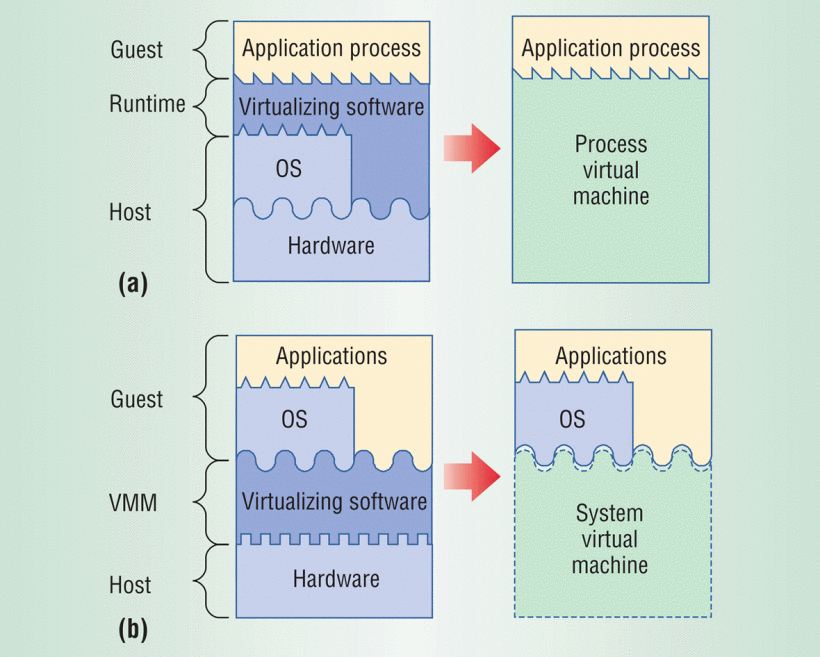
\includegraphics[scale=0.3]{assets/figures/procesvm_vs_sysvm.png}
    \caption[Virtuální stroj v procesu versus systémové virtuální stroje ]{Virtuální stroje v procesech (a) versus systémové virtuální stroje (b) \cite{book:iee:vm_architecture}}
    \label{figure:computer_architecture}
  \end{figure}
  
  
  \subsection{Virtuální stroje v procesech}
  \label{subsection:proces_vm}
  
  Jak již bylo zmíněno tento typ virtuálního stroje poskytuje uživatelským programům virtuální ABI nebo API. Různé implementace těchto virtuálních strojů si kladou za cíl splnění různých kritérií. Některé se snaží
  zajistit přenositelnost mezi různými počítačovými platformami a jiné se snaží optimalizovat instrukce uživatelského programu. Následovat bude stručný výčet jednotlivých typů virtuálních strojů, které spadají 
  do této kategorie.      
  
    \subsubsection*{Virtualizace na úrovni OS}
    \label{subsubsection:os_level_virtualization}
    
    Pro představení prvního zástupce z této rodiny virtuálních strojů nemusíme chodit daleko. Jako virtuální stroj můžeme totiž považovat operační systémy, které umožňují současný běh více procesů najednou. Operační
    systém poskytuje každému procesu iluzi, že na systému běží sám. Z tohoto důvodu je nutné sdílet fyzickou paměť, CPU a jiná HW zařízení mezi běžícími procesy. Operační systém poskytne každému procesu stejně velký
    izolovaný virtuální adresní prostor, který je mapován do fyzické paměti počítače. Procesor se sdílí mezi procesy tak, že dochází k tzv .přepínání kontextu, což znamená uložení všech registrů a načtení registrů
    procesu, který má přidělený procesor. Přístup k ostatním HW zařízením systému je řízen skrze systémové volání operačního systému. Konečně můžeme říct, že OS poskytuje virtuální prostředí pro každý proces v systému.
    
    TODO partišnování zdrojů operačního systému.
    
    \subsubsection*{Emulátory a překladače}
    \label{subsubsection:emulation}
    
    Jak bylo zmíněno výše, některé implementace těchto virtuální strojů jsou zaměřeny na přenositelnost programů mezi jednotlivými počítačovými architekturami. Tyto virtuální stroje zpracovávají instrukce jiné instrukční
    sady než vykonává systém hosta a poté je dynamicky překládají do instrukční sady hosta. Konkrétní implementace by mohla například umožňovat vykonávat programy zkompilované pro architekturu IA-32 na systému s
    architekturou SPARC. Těmto virtuálním strojům říkáme překladače nebo emulátory, jelikož emulují prostředí dostupné na jiných architekturách a mapují ho do architektury hosta.
    
    Techniky překladu instrukcí jsou detailněji popsaný v kapitole \ref{subsubsection:isa_emulation}. Jen pro ukázku si zmíníme techniku interpretace, která jednotlivé instrukce nejprve načte, dekóduje a poté vykoná
    ekvivalentní instrukci nebo sadu instrukcí pomocí instrukční sady hosta.
    
    \subsubsection*{Virtuální stroje v HLL}
    \label{subsubsection:hll_vm}
    
    Virtuální stroje napsané ve vyšších programovacích jazycích přímo navazují na výše popsané téma přenositelnosti mezi platformami. Nevýhoda emulátorů spočívá ve faktu, že se specializují na překlad jedné instrukční sady
    do druhé. Pokud bychom tedy chtěli docílit přenositelnosti mezi všemi platformami, museli bychom vytvořit emulátory pro každou kombinaci instrukčních sad. Jelikož je toto řešení poněkud složité a náročné na
    implementaci, můžeme k vytvoření virtuálního stroje použít právě vyšší programovací jazyky. Virtuální stroj napsaný v nějakém HLL se tedy neopírá o konkrétní architekturu, ale o samotný programovací jazyk a jeho výhody.
    Takto vytvořený virtuální stroj přijímá vlastní jazyk a využívá konkrétního HLL k jeho provádění. Takto je zajištěna přenositelnost programů, které jsou napsané v jazyce virtuálního stroje, mezi systémy, nakterých jsou dostupné
    potřebné knihovny a samotná implementace virtuálního stroje.
    
    Nejznámějším zástupcem této kategorie virtuálních strojů je Java virtual machine od společnosti Sun Microsystems. Tento virtuální stroj provádí instrukce vyššího programovacího jazyka zvaného Java a dnes existuje mnoho
    implementací v nejrůznějších programovacích jazycích. Implementace HotSpot, která je napsaná v jazyce C++ a kterou v dnešní době vyvíjí a udržuje společnost Oracle, je pravděpodobně neznámější a nejvíce využívanou
    implementací JVM.
    
  \subsection{Systémové virtuální stroje}
  \label{subsection:system_vm}
  
  
  
    \subsubsection*{Virtuální počítače}
    \subsubsection*{Virtualizace celého systému}
    \subsubsection*{}
  
  
  \subsection{Definice pojmů}
  \label{definitions}

  Pro potřeby popisu virtualizačních technik si definujeme základní pojmy a entity, které se ve virtuální infrastruktuře vyskytují.

  \textit{Fyzické prostředky} počítače jsou dostupné prostředky a služby poskytované HW počítače. Tyto prostředky určují celkový výpočetní výkon daného stroje.

  \textit{Virtualizační monitor}, \textit{Virtual Machine Monitor - VMM} nebo také \textit{Hypervisor} je softwarová vrstva, která virtualizuje HW prostředky fyzického počítače a přiděluje je
  virtuálním strojům.

  \textit{Virtuální prostředky} jsou virtuální reprezentace fyzických prostředků. Tyto prostředky využívají virtuální stroje skrze VMM. Často tyto prostředky reprezentují pouze nějakou část jejich
  fyzických ekvivalentů. Například část adresního prostoru fyzické paměti nebo určité procento výpočetního času CPU.

  \textit{Host} je HW a SW platforma, která poskytuje virtuálním strojům své fyzické prostředky. Softwarové vybavení hosta obsahuje virtualizační
  monitor a v některých případech může obsahovat i operační systém hosta tzv. \textit{Host OS}

  \textit{Virtuální stroj} nebo \textit{Virtual Machine - VM} je virtualizované prostředí vytvořené virtualizačním monitorem, ve kterém běží operační systém virtuálního počítače nazývaný \textit{Guest OS} společně
  se svými aplikacemi.


\section{Nasazení virtuální infrastruktury}
\label{section:vm_deployment}

Pro přechod k virtuální infrastruktuře serverů existuje v dnešní době několik dobrých důvodů. Jedním z hlavních benefitů virtualizace pro dnešní firmy a organizace je značná finanční úspora. Tato úspora se
projevuje především ve snížení nákladů organizace na pořizování a provoz fyzických zařízení. 

Mezi další benefity virtualizace patří především efektivní využití výpočetních zdrojů, vysoká dostupnost běžících aplikací nebo vytvoření oddělených a nezávislých prostředí pro vývoj, testování a nasazení software.

Výhody zavedení virtuální infrastruktury jsou podrobněji popsány v následujících podkapitolách, které se zabývají základními scénáři pro nasazení virtuální infrastruktury.

\subsection{Konsolidace}
\label{consolidation}

Konsolidace serverů je proces sjednocování systémů z více fyzických serverů na jeden fyzický server, který pro tyto systémy poskytne virtuální prostředí pro jejich běh. Vstupem tohoto procesu je tedy několik systémů na fyzických serverech,
na kterých běží různé aplikace. Vstup procesu je naznačen na obrázku \ref{consolidation_img} vlevo. Výstupem konsolidace je jeden fyzický server s dostatečnými prostředky, na kterém konsolidované systémy běží jako virtuální počítače.
Výstup můžeme vidět na obrázku \ref{consolidation_img} vpravo.

\begin{figure}
    \centering    
    \caption{Konsolidace serverů}
    \label{consolidation_img}
\end{figure}

\subsubsection*{Využití scénáře}

Dnes je zcela běžnou praktikou provozovat jednu aplikaci na jednom dedikovaném serveru. Pokud aplikace využívá jen malé procento výpočetních zdrojů daného serveru, může administrátor sjednotit více takovýchto serverů
do jednoho. Pro organizaci, která vlastní tisíce takovýchto serverů může konsolidace výrazně zmenšit požadavky na prostor, spotřebu energie a provoz fyzických serverů. Správnou konsolidací serverů může společnost docílit
efektivního využití dostupných prostředků a tím výrazně snížit vynaložené finanční prostředky \cite{reasons}.

Rychlý vývoj technologií v oblasti hadware zapříčiňuje rychlé stárnutí některých systémů a přechod ze staršího na nový může být složitý. Obzvláště v případě, kdy systém potřebuje ke svému běhu speciální hadware.
Aby bylo možné provozovat služby poskytované těmito zastaralými systémy, můžeme je spustit jako virtuální počítač na modernějším hadware. Systém se bude chovat stejně jako kdyby běžel na zastaralém hadware, zatímco
výkonost služby může těžit z novější a výkonnější hadwarové vrstvy  \cite{reasons}.

\subsection{Izolace}

Dalším ze scénářů využití virtualizované infrastruktury je izolace aplikací. Proces izolace aplikací spočívá v oddělení dvou a více kritických aplikací běžících na jednom systému do nezávislých virtuálních prostředí.
Vstupem je jeden systém s aplikacemi, které se mohou negativně ovlivňovat. Vstup izolačního scénáře je naznačen na obrázku \ref{izolation} vlevo. Výstupem je několik nezávislých virtuálních počítačů, ve kterých běží
jednotlivé aplikace. Výstup izolace aplikací je ukázán na obrázku \ref{izolation} vpravo.

\begin{figure}
    \centering    
    \caption{Izolace aplikací}
    \label{izolation}
\end{figure}

\subsubsection*{Využití scénáře}

V dnešní době jsou útoky na aplikace vystavené do internetu běžnou záležitostí. Pokud útočník využije nějaké zranitelnosti aplikace, může v některých případech získat kontrolu nad celým systémem. V takovém případě jsou
ohroženy všechny data a aplikace, které na daném systému běží. Vhodným krokem v tomto případě je proto využití virtualizace a rozdělení aplikací do nezávislých prostředí.

Jedním z příkladů ohrožení systému může být útok na výpočetní zdroje. Podstatou útoku je vyčerpání fyzických zdrojů systému, což má za následek nedostupnost jeho služeb a v některých případech i pád celého systému.
Ve virtualizovaném prostředí lze přidělit každému VM pouze určitou část prostředků a tím chránit celý systém před jejich vyčerpáním. V případě napadení jednoho VM sice dojde k jeho vyřazení, ale ostatní VM a jejich služby
mohou dále pokračovat v běhu.

\subsection{Migrace}

Posledním diskutovaným scénářem nasazení virtualizované infrastruktury je migrace. Jedná se o proces přesunutí systému z jednoho počítače na druhý. V rámci virtualizace se budeme bavit o přesouvání systému na počítač s běžícím VMM,
který zprostředkovává virtuální prostředí. Výstupem procesu je systém, který do něj zároveň vstupuje. Rozdíl je v tom, že daný systém na konci procesu běží ve virtuálním prostředí nějakého VMM. Dle typu migrovaného systému můžeme
rozdělit scénář na následující typy.

\subsubsection*{Migrace VM}

Migrací virtuálního stroje se rozumí přesun VM mezi dvěma různými fyzickými stroji s VMM. Tento přesun byl dříve možný pouze v případě když oba stroje měli stejný HW, operační systém a procesor \cite{reasons}.
Tato možnost administrátorovi umožňuje přesouvat virtualizované systémy na výkonnější hosty a tím umožňuje dynamicky regulovat využití fyzických prostředků v závislosti na aktuální zátěži systému.

Další výhodou zavedení virtualizované architektury je zajištění vysoké dostupnosti služeb. Virtualizace umožňuje zajistit redundanci ve smyslu spuštění služby na více serverech najednou. Ve virtualizované architektuře můžou
nastat dva typy selhání. Prvním typem je selhání VM uvnitř VMM. Pokud dojde k selhání některé VM, jiná VM převezme obsluhu požadavků a v minimálním čase dojde k obnovení služby. Druhým typem je selhání celého VMM nebo hosta.
V tomto případě je nutné provozovat více redundantních hostů pro VM, které v případě HW chyby převezmou obsluhu služby.

Proces migrace VM je představen na obrázku \ref{migration1}, kde můžeme vidět konfiguraci před migrací (vlevo) a po provedení migrace VM (vpravo).

\begin{figure}
    \centering    
    \caption{Migrace virtuálního stroje}
    \label{migration1}
\end{figure}

\subsubsection*{Migrace fyzického stoje na VM}

Migrace fyzického stroje na virtuální stroj je proces, kdy dochází k přesunu a virtualizaci systému z fyzického stroje. Vstupem je tedy systém běžící na stroji bez VMM, jak je naznačeno na obrázku \ref{migration2} vlevo. 
Výstupem tohoto procesu je opět virtuální stroj běžící ve virtuálním prostředí VMM.

Virtualizací serverů dochází k uvolňování fyzického HW a stejně jako v případě konsolidace tak společnost může značně ušetřit na nákladech nutných k provozu a správě fyzických serverů. Obecně lze říct, že tento scénář přináší 
podobné benefity jako v případě konsolidace popsané v kapitole \ref{consolidation}.

\begin{figure}
    \centering    
    \caption{Migrace fyzického na virtuální stroj}
    \label{migration2}
\end{figure}

\section{Virtualizační monitor}
\label{section:vmm}

Jak již bylo zmíněno v definici z kapitoly \ref{definitions}, virtualizační monitor je softwarová starající se o virtualizaci fyzických prostředků hosta. Vytváří tedy virtuální prostředí pro běh virtuální počítačů.
Jinak řečeno VMM vytváří iluzi pro každý virtuální počítač, který si myslí že přímo ovládá HW fyzického systému.

V klasickém nevirtualizovaném prostředí se OS stává po zavedení do hlavní paměti hlavním řídícím programem, který spravuje běh aplikací a vyřizuje požadavky aplikací na HW zařízení pomocí ovladačů. Operační systém tedy pracuje
v nejvíce privilegovaném režimu procesoru známého jako \textit{ring 0} a může využívat všechny instrukce instrukční sady.

Druhým případem je prostředí s VMM nebo také virtualizované prostředí. V tomto prostředí přebírá roli hlavního řídícího programu VMM, který je po startu systému zaveden do hlavní paměti. Od té chvíle pracuje VMM v nejvíce privilegovaném
režimu CPU a spravuje všechny hostované OS (guest OS). Ovladače k jednotlivým HW zařízení nyní nejsou součástí těchto OS, ale jsou součástí samotného VMM. Každý OS si sám spravuje vlastní aplikace a chová se jako kdyby nebyl izolován virtualizačním monitorem
ve virtuálním prostředí.\cite{vmm1}

\subsection{Požadavky na VMM}

Z úlohy virtualizačního monitoru při virtualizaci systémů plyne několik základních požadavků, které by měl VMM splňovat. Specifikace těchto požadavků je převzata z \cite{virt2}.

\subsubsection*{Transparentnost}

Operační systém běžící ve virtuálním prostředí virtualizačího monitoru by se neměl dozvědět o existenci VMM ani jiných VM, se kterými ve skutečnosti sdílí prostředky hosta.

VMM tedy zachytává systémové volání operačních systémů na HW zařízení nebo na čtení z paměti a transparentně je vyřizuje. Operační systém virtuálního počítače si tak myslí, že komunikuje přímo s HW. V této fázi VMM využívá 
některých technik virtualizace CPU, paměti nebo I/O zařízení, aby mohl sdílet prostředky mezi virtuální stroje. Některé základní techniky virtualizace jsou popsány v kapitole \ref{virt_techniques}.

\subsubsection*{Izolace}

Virtualizační monitor vytváří virtuální prostředí, které by mělo izolovat jednotlivé instance OS od sebe. Každý virtuální stroj má svůj kontext procesoru i svoji virtuální paměť mapovanou do jiných oblastí fyzické paměti.
Jinak řečeno jednotlivé VM se nemohou vzájemně ovlivňovat svoji činnost a pád jedné VM by neměl ovlivnit činnost ostatních.


\subsubsection*{Ochrana}

Virtualizační monitor by měl být chráněn proti všem vyšším vrstvám virtuální počítačů. Operační systém virtuálního stroje běží v privilegovaném režimu úrovně 1 (ring 1) a VMM běží v nejvíce privilegovaném režimu \footnote[1]{Současné procesory podporují plnou virtualizaci v HW. Mají speciální 
režim ochrany úrovně -1 speciálně pro VMM \cite{virt2}} úrovně 0. Pro operační systém virtuálního počítače to znamená, že nemůže přistupovat do paměti mapované pro VMM a privilegované instrukce vyvolají volání do virtualizačního monitoru, který emuluje jejich chování. 


\subsection{Typy VMM}

V následujících třech podkapitolách jsou představeny tři typické architektury VMM, které se liší ve způsobu přístupu k fyzickým prostředkům systému. Obecně lze tyto způsoby rozdělit na přímý a nepřímý přístup.

\subsubsection*{Nativní VMM}

Virtualizační monitor se nazývá nativní nebo také Bare-Metal, pokud má přímý přístup k HW pomocí vlastních ovladačů. Obvykle se nativní VMM implementuje ve firmwaru počítače nebo jako hlavní program, který se po startu
systému  zavede do hlavní paměti a je mu předáno řízení. Tento přístup poskytuje nejvíce kontroly nad systémem a je také nejefektivnější, protože VMM přístup k HW zařizuje přímo. Architektura nativního VMM je ukázána na 
obrázku \ref{native_vmm}

Pokud hypervisor nepodporuje určité typy procesorů nebo periferních zařízení některých HW plaforem, může softwarové vybavení VMM limitovat přenositelnost na tyto platformy.\cite{vmm1}

\begin{figure}
    \centering    
    \caption{Nativní (Bare-Metal) VMM}
    \label{native_vmm}
\end{figure}

\subsubsection*{Hostovaný VMM}

Druhým typem architektury VMM se nazývá hostovaný, protože využívá ke svému běhu existující a běžící operační systém, který mu poskytuje rozhraní s HW. Virtualizační monitor v tomto případě neobsahuje ovladače k HW, protože jsou
součástí operačního systému hosta. Aby mohl hostovaný VMM správně pracovat, běží některé jeho části (kernel) v privilegovaném režimu procesoru společně s operačním systémem hosta. Požadavky na HW zařízení jsou jádrem VMM přesměrovány
do komponenty VMM, která neběží v privilegovaném režimu. Tato komponenta dále zavolá nativní rozhraní OS a požadavek je vyřízen operačním systémem hosta \cite{vmm1}. Jednotlivé komponenty hostovaného VMM jsou naznačeny na obrázku \ref{hosted_vmm}.

Tento typ virtualizace je v dnešní době velice populární, protože umožňuje používat virtualizaci na systémech s běžícím operačním systémem a to především desktopech. Přenositelnost hostovaného VMM je zcela určena přenositelností 
dané implementace mezi jednotlivými typy OS. Na druhou stranu tento typ VMM není vhodný pro nasazení do prostředí s vysokými výpočetními nároky, jelikož díky další vrstvě mezi HW a VMM není tak efektivní jako nativní VMM.

\begin{figure}
    \centering    
    \caption{Hostovaný VMM}
    \label{hosted_vmm}
\end{figure}

\subsubsection*{Servisní VM}

Některé typy nativních VMM vyžadují pro svoji plnou funkčnost jednu nebo více speciálních instancí VM. Tato instance většinou slouží pro správu VMM a ostatních instancí VM. Nicméně existují i hypervisory, které využívají výhody
existujících OS a především jejich podpory velké škály HW ovladačů. V tomto případě je OS spuštěn ve speciální instanci VM a je společně s jeho ovladači využíván jako komponenta VMM \cite{vmm1}. Tento typ architektury je 
naznačen na obrázku \ref{servise_vmm}.

\begin{figure}
    \centering    
    \caption{VMM se servisním OS}
    \label{servise_vmm}
\end{figure}

\section{Techniky virtualizace}
\label{virt_techniques}

O pár odstavců výše jsme si popsali podstatu virtualizačního monitoru a také jsme si představili jeho základní typy. Nyní se pokusíme popsat techniky a principy, které VMM používá pro práci s HW, aby docílil vytvoření virtuálního prostředí.  

Na chvilku se oprostíme od VMM a podíváme se na HW počítače z pohledu OS. Přesněji chceme vědět, co potřebuje OS ke svému běhu, abychom byli schopni vytvořit virtuální prostředí pro jeho běh. Důležité je zmínit, že chceme na jednom
fyzickém systému provozovat více VM, tedy více instancí OS.

Operační systém je v konečném součtu jenom soubor instrukcí, kterým procesor rozumí a umí je vykonávat. Abychom mohli na fyzickém systému provozovat operační systém nebo jakýkoli jiný program, je nutné aby využíval jen instrukce z
dostupné instrukční sady (ISA) procesoru. Pokud je tento požadavek splněn, může být OS na tomto systému provozován bez dalších opatření. Na druhou stranu pokud požadavek splněn není a instrukce programu jsou napsané v jiné instrukční sadě, 
je nutné tuto sadu emulovat. Jinými slovy musíme zajistit překlad z jedné instrukční sady do druhé. Tomuto tématu se více věnuje kapitola \ref{isa_emulation}. Vedle překladu instrukcí je nutné zajistit sdílení procesoru mezi jednotlivými
virtuálními stroji.

Vedle vykonávání instrukcí potřebuje OS někde uchovávat svoje datové struktury a svůj kód. To samozřejmě vede k hlavní paměti počítače a nutnosti sdílení této paměti mezi virtuálními počítači.

Nemusíme chodit daleko a podobný princip sdílení prostředků mezi více entit můžeme najít v dnešních operačních systémech. V roli virtuálních počítačů si můžeme představit klasické procesy a roli VMM převezme OS, který má za úkol
přidělovat prostředky procesům \cite{virt1}. Stejně jako v případě virtuálních strojů spolu procesy musí sdílet procesorový čas a hlavní paměť, a proto jsou techniky virtualizace počítačů podobné těm, které se používají v OS pro 
souběžný běh více procesů.

V neposlední řadě OS potřebuje ovládat zařízení a periferie připojené k fyzickému systému. K čemu by nám jinak byl počítač, kdybychom nevěděli co nám vlastně říká nebo ho dokonce nemohli ovládat. 

Všechny výše zmíněné problémy musí VMM řešit, pokud chce vytvořit prostředí pro běh více OS na jednom fyzickém stroji. Ve zkratce můžeme říct, že virtualizační monitor musí implementovat multiplexování CPU, virtualizaci paměti,
virtualizaci I/O zařízení a v některých případech i emulaci ISA.

Následujících podkapitoly představují základní techniky, které by měl VMM v nějaké podobě implementovat. Pro lepší pochopení této problematiky si definujeme několik pojmů.

\begin{definition}
Kernel mód
\end{definition}

\begin{definition}
User mod
\end{definition}

\begin{definition}
PC
\end{definition}

\subsection{Virtualizace CPU}

Nyní se opět podíváme na fyzický stroj z pohledu virtualizačního monitoru a na jeho práci s procesorem. Spustit operační systém ve virtuální prostředí nutně musí znamenat, že se nějakým způsobem začnou vykonávat jeho instrukce.
Jelikož OS virtuálního počítače neví o existenci VMM, předpokládá, že je v systému sám a má přímý přístup k HW. Na rozdíl od klasické nevirtualizované architektury není OS hlavním řídícím programem, a proto je nutné, aby VMM obsloužil
volání privilegovaných instrukcí. Dále je třeba zajistit ochranu paměti alokované VMM před neprivilegovaným přístupem. Neprivilegovaný přístup znamená, že se OS virtuálního počítače nebo procesy v něm běžící pokusí přistoupit k paměti, 
která je alokovaná virtualizačním monitorem.

\subsubsection{Režimy ochrany CPU}

Moderní procesory mají 4 režimy ochrany paměti, které se značí čísly od 0 do 3. Nejvyšší režim ochrany má číslo 0 a je označován jako režim kernel. Procesor běžící v tomto režimu má přístup ke všem instrukcím instrukční sady a může přistupovat
k jakékoli paměti. Číslo 3 naopak znamená režim nejnižší ochrany a může využívat jen část instrukční sady, které se někdy přezdívá uživatelská ISA. Tomuto režimu se říká user. Většina operačních systémů používá právě dva výše zmíněné režimy ochrany
a zbylé dva jsou nevyužité.

Operační systémy v nevirtualizované architektuře hrají roli řídícího programu, a proto běží v režimu kernel. Ve virtualizované architektuře tuto roli přebírá VMM, a proto je potřeba, aby běžel v nejvíce privilegovaném režimu. Řešením může být
posunutí OS virtuálního stroje do méně privilegovaného režimu. Například na úroveň 1, zatímco VMM poběží na úrovni 0. Druhým řešením je vytvoření nového režimu ochrany s číslem -1, který bude speciálně pro VMM. Současné procesory řeší ochranu právě tímto
způsobem a podporují plnou virtualizaci v HW \cite{virt2}.

Výsledkem je tedy znemožnění přístupu programů s nižší úrovní ochrany k paměti alokované programem z vyšší úrovně ochrany. Paměť VMM je ve virtualizované architektuře chráněna proti přístupu z OS virtuálního počítače a stejně tak je
chráněna paměť OS virtuálního počítače před přístupem z jeho procesů.

\subsubsection{Multiplexování CPU}

Zjednodušeně můžeme říct, že spuštění virtuálního počítače v prostředí virtualizačního monitoru zařídíme skokem na adresu první instrukce OS.

Pro jednoduchost předpokládejme, že máme k dispozici jedno výpočetní jádro CPU a chceme ho sdílet dvěma virtuálními stroji. Oba virtuální stroje mají svojí instanci OS a běží na nich jejich aplikace. Princip střídání virtuálních strojů
na CPU je velmi podobný s principem střídání běžících procesů v OS. Operační systém provádí tzv. změnu kontextu (context switch), kdy je přerušen běh aktuálního procesu a procesor je přidělen jinému. V případě VMM je nutné provést tzv. změnu stroje (machine switch).
Při tomto procesu dojde nejprve k uložení celého stavu virtuálního stroje, což zahrnuje uložení registrů, PC a na rozdíl od změny kontextu je nutné uložit i aktuální stav HW. Dále je obnoven stav virtuálního stroje, kterému plánovač přidělil procesor
a poté je proveden skok na adresu instrukce uvedené v PC \cite{vmm_book}. Tímto krokem je proces změny virtuálního stroje na CPU dokončen.

V případě systému s více procesorovými jádry je situace velmi podobná. Jelikož je k dispozici více jader CPU, může v jednom okamžiku běžet více VM. Z tohoto důvodu je nutné synchronizovat přístup těchto virtuálních strojů k HW systému.

\subsubsection{Virtualizace privilegovaných instrukcí}

Instrukční sadu procesoru můžeme rozdělit na dvě části. V první části jsou neprivilegované instrukce, které mohou být prováděny v každém režimu ochrany CPU. Tyto instrukce jsou využívány především uživatelskými programy a ve virtualizovaném
prostředí je můžeme přímo provádět na CPU bez nutnosti nějakých opatření. Pokud aplikace nebo OS virtuálního počítače potřebují vykonávat tento typ instrukcí, dojde k jejich provedení na CPU bez nutnosti zásahu VMM.

Druhou částí ISA, jsou tzv. privilegované instrukce, které mohou být prováděny pouze v privilegovaných režimech CPU. Některé privilegované instrukce mohou přímo skryté paměti cache, TLB, vyvolávat přerušení nebo
jiným způsobem ovlivňovat běh systému. Operační systém ve virtualizovaném prostředí nemůže mít možnost vykonávat privilegované instrukce, protože by pak ovládal fyzický systém a od toho je na systému přítomen VMM.
Z tohoto důvodu musí virtualizační monitor nějakým způsobem zachytávat pokusy o vykonávání privilegovaných operací a zajistit jejich správné provedení.

Jedním z případů, kdy VMM musí reagovat na volání privilegované instrukce, je situace, kdy se proces operačního systému snaží provést systémové volání. Příkladem systémového volání může být volání funkce \verb|open()| pro otevření
souboru na disku, volání funkce \verb|write()| pro zápis dat do souboru nebo třeba volání funkce \verb|exec()| pro vytvoření dalšího procesu v systému.

Nejprve se podíváme na to, jak funguje systémové volání v klasických systémech bez virtualizace. Konkrétně se podíváme na architekturu x86, kde se pro dosažení systémového volání používá speciální instrukce přerušení \verb|int| s argumentem 
\verb|0x80|. V ukázce \ref{code:syscall} je zobrazen kód assembleru ze systému FreeBSD \cite{freebsd_syscall}, který spouští systémové volání funkce \verb|open()| pro otevření souboru. Z kódu \ref{code:syscall} je vidět, že volání funkce \verb|open()|
potřebuje tři parametry a to konkrétně mód otevření souboru, příznaky a cestu k souboru na disku. Typ systémového volání je určen díky poslednímu parametru na zásobníku, kterým je v tomto číslo 5 \cite{vmm_book}. A konečně na posledním řádku ukázky se
volá zmíněná instrukce \verb|int|, která vyvolá přerušení.

\begin{lstlisting}[language={[x86masm]Assembler},caption={Systémové volání na FreeBSD},label={code:syscall}]
open:
       push    dword mode
       push    dword flags
       push    dword path
       mov     eax, 5
       push    eax
       int     80h
\end{lstlisting}

Z pohledu virtualizačního monitoru je důležité, co se děje po vyvolání přerušení. Jelikož se jedná o privilegovanou instrukci, dojde k přepnutí procesoru z uživatelského režimu (user) do privilegovaného režimu (kernel) a kontrolu dostane operační systém.
Konkrétně je řízení předáno rutině starající se o obsluhu přerušení, která byla zaregistrována v HW operačním systémem při jeho prvním startu \cite{vmm_book}. Po obsloužení systémového požadavku je řízení vráceno zpět volajícímu procesu.
Posloupnost volání je naznačena v tabulce \ref{table:syscall_nonvirt} společně s přepínáním režimu ochrany procesoru.

\begin{table}
    \centering        
    \begin{tabularx}{\textwidth}{XXX}
    Proces & Hardware & Operační systém \\
    \hline    
    1. \textit{Systémové volání:} && \\ Vyvolání přerušení; && \\
    & 2. \textit{Kernel mód:} & \\ & Skok na obsluhu přerušení; & \\
    && 3. \textit{Obsluha přerušení:}  \\ && Dekódování přerušení a spuštění odpovídající rutiny OS;\\ && Návrat z OS; \\
    & 4. \textit{User mód:} & \\ & Návrat z obsluhy; & \\
    5. \textit{Obnova běhu;} && \\
    \end{tabularx}
    \caption[Sytémové volání bez virtualizace]{Sytémové volání bez virtualizace \cite{vmm_book}}
    \label{table:syscall_nonvirt}
\end{table}

Je logické, že případě virtualizace bude nutné přidat několik kroků do posloupnosti volání. Rozdílem oproti předchozímu případu je fakt, že OS nemá nad systémem plnou kontrolu a neběží v plně privilegovaném režimu. Tuto funkci nyní plní VMM, který
má v HW zaregistrovanou rutinu pro obsluhu přerušení. Pokud tedy nějaký uživatelský proces chce provádět systémové volání, bude postupovat stejně jako v předchozím případě. Nicméně zpráva o přerušení se nedostane k OS ale k VMM, jak je naznačeno v
druhém kroku v tabulce \ref{table:syscall_virt}. Virtualizační monitor nemůže přímo vyřídit systémové volání, protože mu nerozumí a neví co má dělat (není OS). Tuto funkci plnil operační systém a jeho rutina pro obsluhu přerušení. Jak již bylo zmíněno,
při prvním startu OS se systém pokusí registrovat v HW rutinu pro obsluhu přerušení, což je ale privilegovaná operace \cite{vmm_book}. Tento pokus VMM odchytí a ke každému běžícímu OS si zaznamená adresu těchto rutin. Virtualizačnímu monitoru tedy stačí
spustit rutinu korespondující OS v méně privilegovaném režimu a počkat na její dokončení. V okamžiku ukončení obsluhy systémového OS opět provede privilegovanou instrukci a řízení je předá zpět VMM, jak je ukázáno ve čtvrtém kroku tabluky \ref{table:syscall_virt}.
Konečně VMM přepne procesor do uživatelského režimu a vrátí řízení zpět uživatelskému programu, čímž je systémové volání ukončeno. V tabulce \ref{table:syscall_virt} jsou z důvodu úspory místa vynechány operace HW, které přepínají režimy procesoru.

Z obou tabulek je patrné, že při virtualizaci se musí vykonat více kroků, čímž se zvyšuje doba vykonávání privilegovaných instrukcí a to může mít za následek zhoršení výkonu systému \cite{vmm_book}.

\begin{table}
    \centering    
    \begin{tabularx}{\textwidth}{XXX}
    Proces & Operační systém & Virtualizační monitor \\
    \hline
    1. \textit{Systémové volání:} && \\ Vyvolání přerušení; && \\
    && 2. \textit{Obsluha přerušení:} \\ && Skok na obsluhu přerušení odpovídajícího OS (snížení privilegií) \\    
    & 3. \textit{Obsluha přerušení:} & \\ & Dekódování přerušení a obsloužení systémového volání; & \\ & Návrat z OS; & \\
    && 4. \textit{Obsluha ukončena:} \\ && Provedení reálného návratu;\\
    5. \textit{Obnova běhu;} &&\\
    \end{tabularx}

    \caption[Sytémové volání s virtualizací]{Sytémové volání s virtualizací \cite{vmm_book}}
    \label{table:syscall_virt}
\end{table}


\subsubsection{Emulace instrukční sady}
\label{subsubsection:isa_emulation}

Doposud jsme se bavili o situaci, kdy stroje běžící ve virtualizovaném prostředí zpracovávaly instrukce stejné architektury jako host. Nyní se krátce podíváme na situaci, kdy virtuální stroje zpracovávají instrukce
jiné architektury než fyzický stroj.

V tomto případě procesor nerozumí instrukcím VM a je nutné zajistit překlad z jedné ISA do druhé. Tato technika se nazývá emulace instrukční sady a spočívá v navození iluze, že virtuální stroj běží
na HW podporující jeho instrukční sadu. 



\begin{itemize}
 \item Přímá interpretace
 \item Binární překlad
 \item Inkrementální binární překlad za běhu
\end{itemize}


\cite{virt3}



\subsection{Virtualizace Paměti}
\subsection{Virtualizace I/O zařízení}


